\chapter{Normalising the Typed Lambda Calculus}
\label{chap:typednbe}

In this chapter, we translate an Agda implementation of NbE developed by Andras Kovacs \cite{AgdaNbe} for the STLC into Haskell.

\section{Target Syntax}

% TODO: Colour for polymorphic type variable in certain blocks

We construct the set of the simply typed normal terms \code{NormalForm} by combining the approach seen for the untyped terms in Chapter \ref{chap:untypednbe} with the GADT syntax from Chapter \ref{chap:typedlamadacalculus} to ensure \code{NormalForm}'s inhabitants are well-typed.

\begin{lstlisting}
    data NormalForm :: [Ty] -> Ty -> * where
        NormalNeutral :: NeutralForm ctx ty -> NormalForm ctx ty
        NormalLam     :: NormalForm (arg : ctx) result -> NormalForm ctx (arg :-> result)    

    data NeutralForm :: [Ty] -> Ty -> * where
        NeutralVar :: Elem ctx ty -> NeutralForm ctx ty
        NeutralApp :: NeutralForm ctx (arg :-> result) -> NormalForm ctx arg 
                   -> NeutralForm ctx result

\end{lstlisting}

% TODO: Justify why V has context (need to reify, example, normalise identity), describe what we need



% TODO: First evaluation problem - returning correct semantic context, lambda has different syntax
% - Solved for us by Andras

% TODO: Correspondence with untyped env, Motivate need for tracking type, ctxV

\section{Order Preserving Embeddings}

Following Kovacs' implementation, before we can define the semantic set we need a datatype to represent Order Preserving Embeddings (OPEs) on contexts.

\begin{lstlisting}
    data OPE :: [Ty] -> [Ty] -> * where
        Empty :: OPE '[] '[]
        Drop  :: OPE ctx1 ctx2 -> OPE (x : ctx1) ctx2
        Keep  :: OPE ctx1 ctx2 -> OPE (x : ctx1) (x : ctx2)
\end{lstlisting}

A value of type \code{OPE a b} is a proof that the list of types \code{b} is a subsequence of \code{a}. The three constructors of \code{OPE} correspond to the different ways of constructing such a proof. The \code{Empty} constructor corresponds to the trivial statement that the empty list contains itself. Given a proof that \code{ctx2} is embedded in \code{ctx1}, the \code{Drop} constructor extends the proof to show that \code{ctx2} is embedded in \code{x:ctx1}, and the \code{Keep} constructor extends the proof to show that \code{x:ctx2} is embedded in \code{x:ctx1}. For example, \code{Drop (Keep Empty))} could have the type \code{OPE '[BaseTy :-> BaseTy, BaseTy] '[BaseTy]}. 

From a programs as proof perspective, \code{OPE} is a binary relation on the set of contexts.

% Q: Order changes dB Indices if drop from middle?

% TODO: Motivate why need in terms of eval, read Andras Paper

\section{Semantic Set}

\begin{figure}[h]
    \centering
    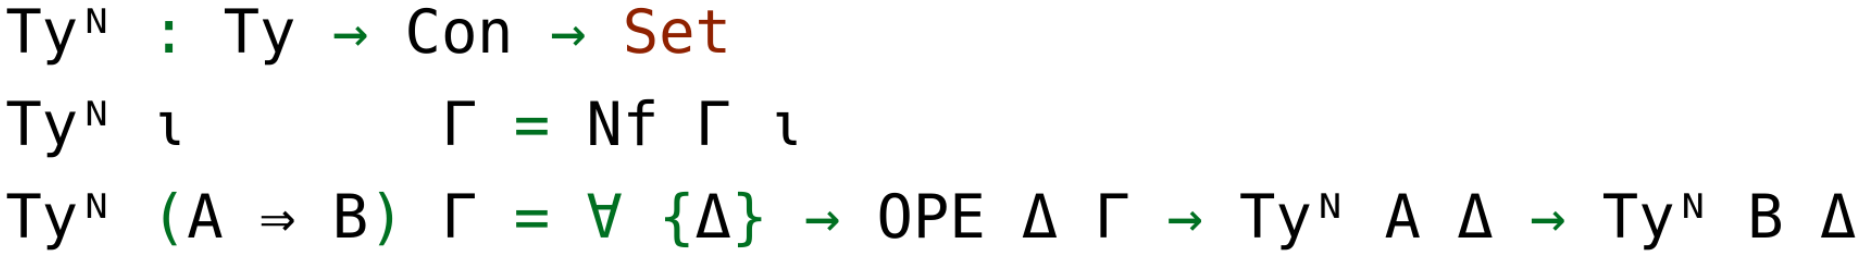
\includegraphics[width=0.7\textwidth]{./images/typed_semantic_set.png}
    \caption{Agda implementation of the typed semantic set from \cite{AgdaNbe}}
    \label{fig:agdaSemanticSet}
\end{figure}

% Differences between Haskell and Agda (presentation)

% The \code{normalise} function should return a \code{NormalForm} with the same type and typing context as the original term, so should have the type signature \code{Expr ctx ty $\rightarrow$ NormalForm ctx ty}. Because \code{reify} is a pure function of the semantic set \code{V}, this set must also be indexed by the typing context and type of the expression to preserve the type information needed to verify a term is well-typed (as seen in the kind signature below). 

In Andras Kovacs' implementation of NbE \cite{AgdaNbe}, the type of the semantic set is determined by the function $\text{Ty}^\text{N}$. This function takes the type and context of an expression as values, and returns the type of the corresponding semantic set, where \code{Set} can be thought of as kind \code{*}. In Haskell we do not have a way to directly express a function which takes values and returns types. Instead we define the GADT \code{V} which represents the typed semantic set.

\begin{lstlisting}
    data V :: [Ty] -> Ty -> * where 
        Base :: NormalExpr ctx 'BaseTy -> V ctx 'BaseTy
        Function :: (forall ctx' .  OPE ctx' ctx -> V ctx' arg -> V ctx' result) 
                 -> V ctx (arg :-> result)
\end{lstlisting}

\code{V} is indexed by a context of kind \code{[Ty]} and a type of kind \code{Ty}, which were value-level function arguments in Figure \ref{fig:agdaSemanticSet}. \code{V} is necessarily indexed by these parameters at the type level since \code{normalise} should return a normal form with the same context and type as the given syntactic expression. \code{reify} is a pure function of the semantic set, so \code{V} must preserve this type-level information. 

$\text{Ty}^\text{N}$ pattern matches on the type argument and is defined in two cases: a base type case and a function case, where the Agda implementation uses $\iota$ for \code{BaseTy}. In our implementation the expression type is not given as a value-level argument that can be pattern matched on, so instead we use constructors to emulate a similar behaviour. From the return type of the constructors we see that values of \code{V} with type \code{BaseTy} can only be created by the \code{Base} constructor. Thus, if we are given a value of type \code{V ctx 'BaseTy}, GHC can deduce the value takes the form \code{Base n} where \code{n :: NormalExpr ctx Expr}. \code{n} is an inhabitant of the type returned by the Agda implementation in the base type case. 
Similarly, given a value of type \code{V ctx (A :-> B)}, GHC can deduce that the value must have the form \code{Function f}, since only the \code{Function} constructor can produce semantic values with function type. Again, we can extract a semantic value of the correct type since the type of \code{f} is exactly the type specified by the function type case of $\text{Ty}^\text{N}$. Thus, we have successfully mimicked the behaviour of $\text{Ty}^\text{N}$ in Haskell.

% TODO: Limitations of above technique

The argument to the \code{Function} constructor has following the type signature.
\begin{lstlisting}
    forall ctx' . OPE ctx' ctx -> V ctx' arg -> V ctx' result 
\end{lstlisting}

By default, in GHC, there is only have one “level” of polymorphism, where type variables are implicitly universally quantified. However, as seen in Figure \ref{fig:agdaSemanticSet}, we want to treat \code{ctx} as fixed, before quantifying over \code{ctx'}, where we use \code{ctx} instead of $\Gamma$ and \code{ctx'} instead of $\Delta$.
% Those with OPE to original context
To achieve this we use higher-ranked polymorphism with the explicit \code{forall} syntax to delay the quantification of \code{ctx'} until after \code{ctx} has been bound. To enable higher ranked polymorphism, we use the \code{Rank2Types} extension. 

The \code{OPE} parameter acts as a precondition requiring a proof that \code{ctx'} contains \code{ctx}, so intuitively this type quantifies over all contexts containing \code{ctx}.

% TODO: Justify use of OPE further? 

\section{Evaluation}

In this section we implement the typed \code{eval} function.

\subsection{Environment}

% TODO: Relation to agda

As in the untyped implementation of NbE, during evaluation we need an environment to track bound variables and their associated semantic values. Since our variables have the same structure as de Bruijn indices, it suffices to use a list as the environment, where the $n$th element of the list corresponds to the variable with de Bruijn index $n$.

% TODO: Motivated by the variable case
% Need extra typing info

\begin{lstlisting}
    data Env :: [Ty] -> [Ty] -> * where
        EmptyEnv :: Env '[] ctxV
        ConsEnv  :: Env ctx ctxV -> V ctxV ty -> Env (ty : ctx) ctxV
\end{lstlisting}

From the constructors, we see that the \code{Env} GADT has the same value-level structure as the standard Haskell list. However, we have used GADT syntax to enforce additional restrictions on the types of the elements in the environment. From the kind signature, we see that \code{Env} is indexed by two typing contexts. From the constructor types, we see that the first of these tracks the types of the semantic elements stored in the environment. The second typing context is the typing context shared by all semantic values stored in the environment. The motivation for indexing \code{Env} by these typing contexts is due to \code{envLookup} function defined below in \ref{subsect:typedetaExpandCase}.


% Why do ctxs have to match?

\subsection{Variable Case}
\label{subsect:typedetaExpandCase}

Now that we have defined the environment, we can begin implementing the evaluation function \code{eval}.

\begin{lstlisting}
    eval :: Env ctx ctxV -> Expr ctx ty -> V ctxV ty
\end{lstlisting}

As before, we pattern match on each of the three expression constructors. We start with the variable case.

\begin{lstlisting}
    eval env (Var n) = envLookup n env
        where
            envLookup :: Elem ctx ty -> Env ctx ctxV -> V ctxV ty 
            envLookup Head     (ConsEnv _    v) = v
            envLookup (Tail n) (ConsEnv tail _) = envLookup n tail
\end{lstlisting}

As in the untyped case, for variables we lookup the semantic value associated with the bound variable from the environment. Since variables are indexed by an \code{Elem} value, \code{envLookup} takes an \code{Elem} value and returns the associated semantic value.

The additional type information encoded in \code{Env} allows us to make guarantees about the lookup. Since \code{n} is a value of type \code{Elem ctx ty}, we know that \code{ty} exists somewhere in the list \code{ctx}. Since \code{Env} is also indexed by the same context \code{ctx}, which tracks the types of the semantic values in the environment, it is guaranteed that the semantic value at the corresponding de Bruijn index exists in the environment with type \code{ty}. Thus, \code{envLookup} doesn't have to handle the case where the variable is not in the environment like in the untyped implementation; the types guarantee that all variables possible in the context \code{ctx} are bound in the environment.

Since all semantic values in the environment have the same typing context \code{ctxV}, we can also be sure that the returned semantic value has the context \code{ctxV}.

Note that \code{envLookup} does not pattern match on the \code{EmptyEnv} case. The types ensure that this case is never required since \code{EmptyEnv} has type \code{Env '[] ctxV}, and there are no inhabitants of the type \code{Elem '[] x} for any \code{x}. Here \code{Elem ctx ty} acts like a pre-condition on \code{envLookup}.

% TODO: Why return into ctxV?

\subsection{Lambda Case}
\label{subsect:typedEvalLamCase}

Before implementing the lambda case of \code{eval} we define the function \code{strengthenEnv} with type signature \code{OPE ctxV' ctxV -> Env ctx ctxV -> Env ctx ctxV'}. \code{strengthenEnv} takes an \code{OPE ctxV' ctxV} and an environment, and returns the same environment where each semantic value has the expanded context \code{ctxV'}. To implement \code{strengthenEnv}, we first build a series of functions for strengthening each constituent part of a semantic value.

\begin{lstlisting}
    strengthenElem :: OPE strong weak -> Elem weak ty -> Elem strong ty
    strengthenElem (Drop ope) v        = Tail (strengthenElem ope v)
    strengthenElem (Keep ope) (Tail v) = Tail (strengthenElem ope v)
    strengthenElem (Keep ope) Head     = Head
\end{lstlisting}

First we strengthen \code{Elem} values which index variables. We use the naming convention \code{OPE strong weak} since \code{strong} contains at least as many bindings as \code{weak}. 
We can perform this context strengthening since if \code{ty} is an element of the context \code{weak}, then it is also an element of any context \code{strong} containing \code{weak}.

% TODO: Rephrase above

% TODO: Explain cases?

\begin{lstlisting} 
    strengthenNormal :: OPE strong weak -> NormalExpr weak ty -> NormalExpr strong ty
    strengthenNormal ope (NormalNeutral n) = NormalNeutral (strengthenNeutral ope n)
    strengthenNormal ope (NormalLam n)     = NormalLam (strengthenNormal (Keep ope) n)

    strengthenNeutral :: OPE strong weak -> NeutralExpr weak ty -> NeutralExpr strong ty
    strengthenNeutral ope (NeutralVar n)   = NeutralVar (strengthenElem ope n)
    strengthenNeutral ope (NeutralApp f n) = NeutralApp (strengthenNeutral ope f) 
                                                        (strengthenNormal ope n) 

\end{lstlisting}

\code{strengthenNeutral} and \code{strengthenNormal} strengthen entire expressions. Intuitively any well-typed expression in one context should also be well-typed in any larger context containing original, since adding variable bindings will not invalidate existing type judgements. \code{strengthenNormal} essentially encodes the weakening property for the normal form subset of the STLC. 

In the \code{NormalLam} case, type refinement guarantees that the context for the body of the lambda binds an additional variable. Hence, we have to expand the given OPE with an additional \code{Keep}. In the \code{strengthenNeutral} case we use \code{strengthenElem} to point variables to their updated de Bruijn indices in the expanded context.

\begin{lstlisting}
    strengthenV :: OPE strong weak -> V weak ty -> V strong ty
    strengthenV ope (Base nf)    = Base (strengthenNormal ope nf)
    strengthenV ope (Function f) = Function f' 
        where
            f' ope' v = f (composeOPEs ope ope') v

    composeOPEs :: OPE b c -> OPE a b -> OPE a c
    composeOPEs v        Empty    = v
    composeOPEs v        (Drop u) = Drop (composeOPEs v u)
    composeOPEs (Drop v) (Keep u) = Drop (composeOPEs v u)
    composeOPEs (Keep v) (Keep u) = Keep (composeOPEs v u)
\end{lstlisting}

\code{strengthenV} takes an \code{OPE} and a value of the semantic set, and strengthens the semantic value according to the given \code{OPE}.

If \code{ope' :: strongest strong} and \code{v :: V strongest arg}, then to satisfy the type restrictions of the semantic set in the \code{Function} case, we need to apply \code{v} to \code{f} with an \code{OPE} of type \code{OPE strongest weak}. We produce such an \code{OPE} using the \code{composeOPEs} function, which implements transitivity for two \code{OPE}s.

% Q: Deeper explanation required?
% Q: Is this like weakening for semantics?

However, GHC automatically infers that \code{f' :: OPE Any strong -> V Any arg -> V Any result}, which leads to a failure to compile at type-checking. This error occurs since all the contexts which GHC has inferred as \code{Any} must be the same to satisfy type-checking, and since values of type \code{Any} can be different, GHC cannot deduce necessary type equalities between these contexts. 

\begin{lstlisting}
    strengthenV :: OPE strong weak -> V weak ty -> V strong ty
    strengthenV ope                      (Base nf) = Base (strengthenNormal ope nf)
    strengthenV (ope :: OPE strong weak) (Function 
        (f :: forall strong . OPE strong weak -> V strong arg -> V strong result)) 
        = Function f' 
            where
                f' :: OPE strongest strong -> V strongest arg -> V strongest result
                f' ope' = f (composeOPEs ope ope')
\end{lstlisting}

To resolve this issue we use type annotations, which are enabled by the \code{ScopedTypeVariables} extension. \code{ope :: OPE strong weak} binds the type variables \code{strong} and \code{weak} in the body of the case. We also bind the type variables for the constructor argument \code{f}. We can then use these bound variables to specify the type of \code{f'}, where we explicitly declare that the contexts inferred as \code{Any} must be the same context \code{strongest}. With this additional type information, type-checking succeeds and the program compiles.

\begin{lstlisting}
    strengthenEnv :: OPE ctxV' ctxV -> Env ctx ctxV -> Env ctx ctxV'
    strengthenEnv _   EmptyEnv         = EmptyEnv
    strengthenEnv ope (ConsEnv tail v) = ConsEnv (strengthenEnv ope tail) (strengthenV ope v)
\end{lstlisting}

\code{strengthenEnv} maps over the elements of the environment, strengthening each one in turn with the \code{strengthenV} function.

Now we are ready to implement the lambda case of the \code{eval} function.

\begin{lstlisting}
    eval env (Lam body) = Function f 
        where
            f ope v = eval (ConsEnv (strengthenEnv ope env) v) body
\end{lstlisting}

As in the untyped implementation, in the lambda case \code{eval} returns a semantic function that maps from a semantic argument \code{v} to the evaluated body of the lambda. We evaluate the body in an updated environment where we have bound the variable \code{Var Head} to \code{v}. However, if \code{ope :: ctxV' ctxV} then \code{v} has the context \code{ctxV'} whereas all the elements of \code{env} have context \code{ctxV}, so we cannot immediately add \code{v} to \code{env}. Instead, we have to strengthen the contexts of all the elements of the \code{env} using the given \code{ope} argument and \code{strengthenEnv}, which yields the strengthened environment of type \code{Env ctx ctxV'}. Now the contexts of the elements of the modified environment match the context \code{ctxV'} of \code{v}, so we can add \code{v} to the modified environment. 

As in the \code{Function} case of \code{strengthenV}, the type of \code{f} that GHC infers is 

\begin{lstlisting}
    OPE Any ctxV -> V Any arg -> V Any result
\end{lstlisting}

which is too general and causes compilation to fail at type-checking.

\begin{lstlisting}
    eval (env :: Env ctx ctxV) (Lam (body :: Expr (arg:ctx) result)) = Function f 
        where
            f :: OPE ctxV' ctxV -> V ctxV' arg -> V ctxV' result
            f ope v = eval (ConsEnv (strengthenEnv ope env) v) body
\end{lstlisting}

Once we have annotated the argument types, type-checking and compilation succeed.

\subsection{Application Case}
\label{subsect:typedEvalAppCase}

\begin{figure}[h]
    \centering
    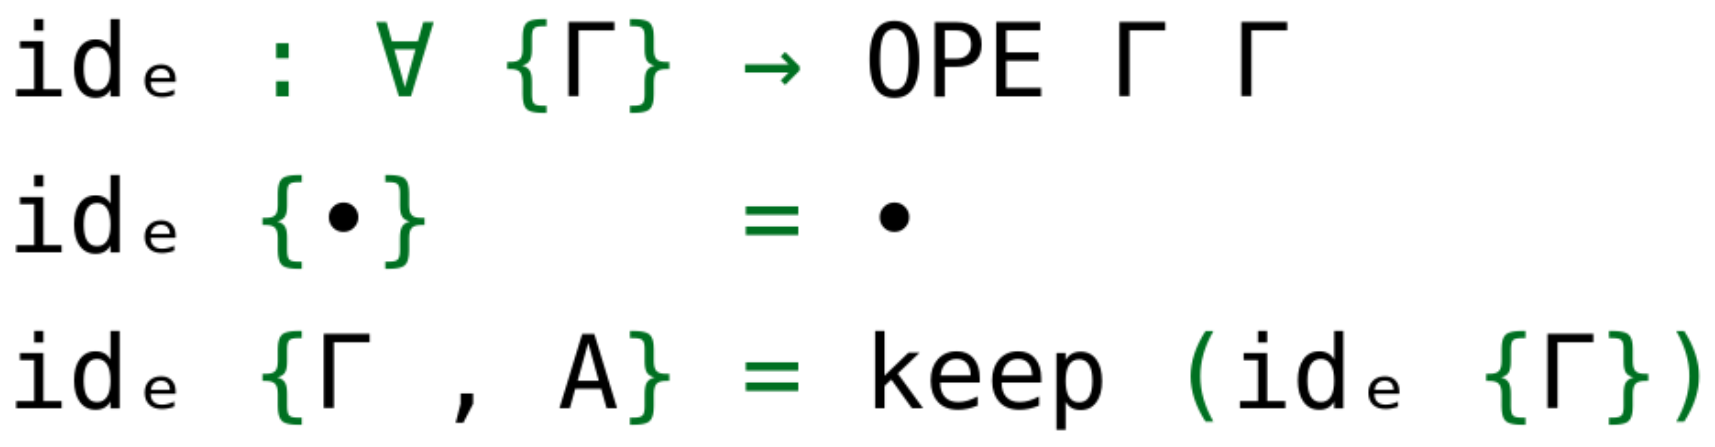
\includegraphics[width=0.38\textwidth]{./images/agda_id_ope.png}
    \caption{Agda implementation of the identity OPE from \cite{AgdaNbe}}
    \label{fig:agdaIdOPE}
\end{figure}

Before implementing the lambda case of \code{eval}, we need to define the identity \code{OPE} function from Figure \ref{fig:agdaIdOPE} in Haskell. This function pattern matches on the type-level context $\Gamma$ and produces the identity \code{OPE} proving that $\Gamma$ is contained in $\Gamma$. This is known as a dependent pattern match, as the result of the function is dependent of the type of its arguments. In Haskell, standard functions cannot pattern match on types, so we use an alternative construction, inspired by the singleton pattern \cite{singletons}, to pattern match at the type level.

% IDEAS: Functionality, Agda implementation, why not in Haskell, solution, how works (runtime-lookup), limitations?

% only well-typed for lists of types (not other type level lists) by OPE parameter

\begin{lstlisting}
    class SingContext ctx where
        idOpe :: OPE ctx ctx

    instance SingContext '[] where
        idOpe = Empty

    instance (SingContext xs) => SingContext (x:xs) where
        idOpe = Keep idOpe
\end{lstlisting}

We create a class \code{SingContext} with a single method \code{idOpe}, which will return the identity \code{OPE} for the context \code{ctx}. We then use class instances to pattern match on the type of \code{ctx}. In the empty context case, \code{idOpe} returns the \code{Empty} \code{OPE}. In the \code{x:xs} case, we require that the type \code{xs} has a \code{SingContext} instance which grants us the ability to use the \code{idOpe :: OPE xs xs} function in the instance definition. Applying the \code{OPE} for the tail of the list to the \code{Keep} constructor produces the identity \code{OPE} for the whole list. 

The class instances essentially form a map from types to implementations of \code{idOpe}. Since \code{ctx} is a type variable that might not be known until runtime, the process of resolving the correct implementation to use could take place at runtime. This is surprising given that without extensions, GHC erases all type information during compilation. 

% TODO: Talk more on this? - perfomance impact of carrying around type information

% Q: dynamic Type-level pattern matching due to DataKinds?

% Q: Inlining only possible because one class type variable?

We are now ready to define the application case of the \code{eval} function

\begin{lstlisting}
    eval env (App f n) = appV (eval env f) (eval env n) 
        where
            appV (Function f') n' = f' (idOPEFromEnv env) n'

            idOPEFromEnv :: (SingContext ctxV) => Env ctx ctxV -> OPE ctxV ctxV
            idOPEFromEnv _ = idOpe 
\end{lstlisting}

We first evaluate both terms of the application into the semantics, and then perform application at the semantic level using the \code{appV} function. 

From the definition of \code{Function}, we can evaluate our function with a semantic argument in any context stronger than \code{ctxV}, where the \code{OPE} argument is a witness to the stronger context.
% TODO: Rephrase above
Since \code{n'} has the same context \code{ctxV} as \code{Function f'}, we evaluate the semantic function \code{f'} at \code{ctxV} by choosing the \code{OPE} of type \code{OPE ctxV ctxV}. We produce such a value using the \code{idOPEFromEnv} function. This function takes an environment but throws away the value since the only information needed to produce the \code{OPE} is the type-level semantic context \code{ctxV}. The \code{SingContext ctxV} constraint awards us the \code{idOPE :: OPE ctxV ctxV} function, which handles the type level pattern match on \code{ctxV} and produces the identity \code{OPE} of \code{ctxV}. 

To ensure that \code{ctxV} is an element of the \code{SingContext} class, we add the same constraint to \code{eval}'s type signature to give \code{eval :: (SingContext ctxV) => Env ctx ctxV -> Expr ctx ty -> V ctxV ty}. 
Without this additional constraint, GHC cannot be sure that \code{ctxV} is a member of the \code{SingContext} class, so the constraint on \code{idOPEFromEnv} is not satisfied, and compilation fails. However, any function that uses \code{eval} now also has to prove that \code{ctxV} has a \code{SingContext} instance to satisfy \code{eval}'s constraint. By adding class constraints, we implicitly propagate this guarantee back through the call-stack. Eventually we reach a point where the \code{ctxV} variable is instantiated with a concrete type that GHC can infer has a \code{SingContext} instance, which it can't do for arbitrary type variables like \code{ctxV}. This adds boilerplate code to type signatures, but is necessary to ensure type-checking succeeds and does not impact the implementation of the functions themselves. For successful compilation we would need to retrofit previously defined code with the necessary class constraints, but since these constraints do not affect the operation of functions, we omit them for brevity.

% TODO: Include code link

Since it is guaranteed by the \code{Expr} GADT that \code{f} has a function type, it is guaranteed by \code{eval} that its semantic interpretation \code{eval env f} also has a function type. Thus, we only need to define the \code{Function} case of \code{appV}, since \code{Function} is the only constructor of \code{V} that can produce a semantic value of function type. In fact, when the \code{appV (Base v) a = ...} case is included, GHC detects that the pattern match is redundant and issues an \code{Inaccessible code} warning at compile time. 

% TODO: Discuss why relevant

\section{Reification}

In this section we implement the \code{reify} function, which takes elements of the semantic set to their canonical well-typed normal forms. 

\begin{lstlisting}
    reify :: V ctx ty -> NormalForm ctx ty
    reify (Base nf) = nf
\end{lstlisting}

Since semantic values with type \code{BaseTy} are normal forms, \code{reify} returns the corresponding normal form \code{nf}.

\begin{figure}[h]
    \centering
    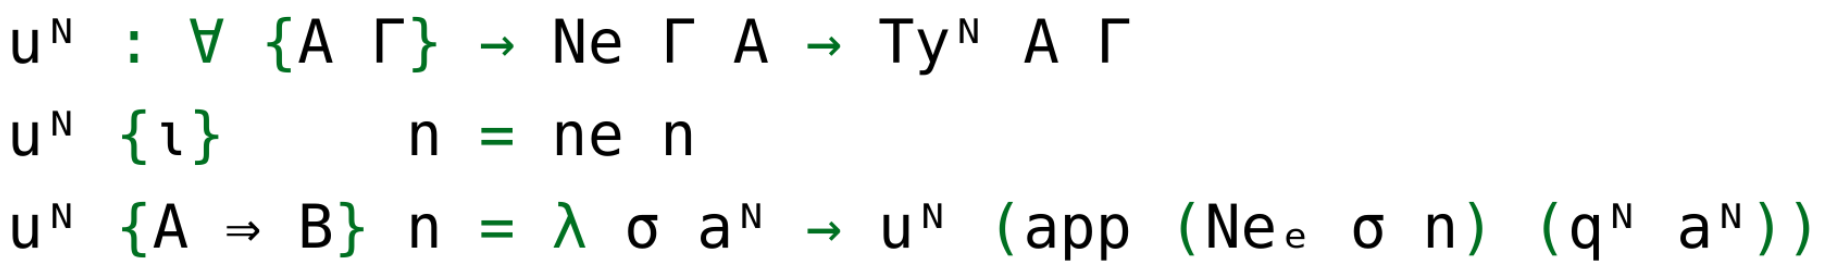
\includegraphics[width=0.7\textwidth]{./images/agda_eta_expand.png}
    \caption{Agda implementation of \code{etaExpand} from \cite{AgdaNbe}}
    \label{fig:agdaEtaExpand}
\end{figure}

It would be desirable to normalise expressions into $\eta$-expanded normal form, where all the arguments of expressions with function type are abstracted. \code{etaExpand} is the function responsible for evaluating syntactic expressions into $\eta$-expanded semantic expressions. To implement \code{etaExpand} we follow the Agda definition in Figure \ref{fig:agdaEtaExpand}, where we use \code{etaExpand} for $\text{u}^\text{N}$ and \code{reify} for $\text{q}^\text{N}$. $\text{u}^\text{N}$ pattern matches on the type \code{A} at the type-level. Since this is not possible directly in Haskell, we use the same class instance trick from the application case of \code{eval}. 

\begin{lstlisting}
    class SingTy ty where
        etaExpand :: NeutralForm ctx ty -> V ctx ty

    instance SingTy 'BaseTy where
        etaExpand n = Base (NormalNeutral n)

    instance (SingTy result) => SingTy (arg :-> result) where
        etaExpand (n :: NeutralForm ctx (arg :-> result)) = Function f 
            where
                f :: OPE ctx' ctx -> V ctx' arg -> V ctx' result
                f ope v = etaExpand (NeutralApp (strengthenNeutral ope n) (reify v))  
\end{lstlisting}

We create a class \code{SingTy} with a single function \code{etaExpand}, where the type of the neutral form is bound to the type \code{ty} parameterising the class. The \code{'BaseTy} instance is used when the argument \code{n} is an expression of type \code{BaseTy}. In the body of the instance, GHC infers that \code{n :: NeutralForm ctx 'BaseTy}, which allows us to apply the \code{Base} constructor. The \code{:->} instance is used when \code{n} has a function type. In this case we use type annotations again since the automatically inferred type of \code{f} is too general for successful compilation. This annotation also shows us that in the function case, GHC is able to infer that \code{n :: NeutralForm ctx (arg :-> result)}. In this instance, \code{etaExpand} returns a function, which will eventually be reified into a lambda. However, the body of this function may itself may require $\eta$-expansion, depending on the type \code{arg} of the argument \code{v}. Since the \code{NeutralApp} constructor creates a neutral value of type \code{result}, \code{etaExpand} requires that \code{result} also has a \code{SingTy} instance in the instance declaration.

In the untyped implementation of NbE, evaluation and reification take place in two distinct phases. However, from the definition of \code{etaExpand} we see that in the typed implementation, expressions are bounced back and forth between syntactic and semantic representations. This makes the implementation more difficult to reason about, but is a necessary trade-off to achieve the additional type security and features such as $\eta$-expansion that the typed implementation provides.

\begin{lstlisting}
    class SingContext ctx where
        idOpe :: OPE ctx ctx
        bindOpe :: OPE (arg:ctx) ctx
        bindOpe = Drop idOpe
\end{lstlisting}

We extend the existing class \code{SingContext} to include \code{bindOpe}, which produces an \code{OPE} from a given context \code{ctx} to one where we have bound a new variable \code{arg:ctx}. Since \code{bindOpe} is defined the same way in both the \code{Empty} and \code{(:)} cases, we set a default implementation in the class definition and leave the individual instances unaltered. 

\begin{lstlisting}
    reify (Function f) = NormalLam (reify (f extendedOpe boundVar)) 
        where
            boundVar = etaExpand (NeutralVar Head)

            extendedOpe = extendOpe (Function f)

            extendOpe :: (SingContext ctx) => V ctx ty -> OPE (arg:ctx) ctx
            extendOpe _ = bindOpe 
\end{lstlisting}

To reify a function \code{f :: OPE ctx' ctx -> V ctx' arg -> V ctx' result}, we evaluate the \code{f} at a semantic bound variable, and reify the result (which represents the body of the function \code{f}). \code{boundVar} has the type \code{V (arg:ctx) arg}, so we use the \code{extendedOpe} function to produce an \code{OPE} for a context where we have bound an additional variable of type \code{arg} in the context. All instances of the argument in the body of \code{f} are replaced with \code{etaExpand (NeutralVar Head)}. From the definition of \code{etaExpand}, we see that if \code{NeutralVar Head} has type \code{BaseTy}, \code{etaExpand} can immediately evaluate the variable into the semantic set. On the other hand, if \code{NeutralVar Head} has a function type, \code{etaExpand} evaluates to a function which waits for an argument to be supplied before continuing evaluation of the variable.

The other section of the program where we evaluate a semantic function \code{f} is the application case of \code{eval} (see Section \ref{subsect:typedEvalAppCase}). These cases motivate the use of \code{OPE}s, since in the application case we need to evaluate \code{f} in the same context as the semantic value, whereas in this case we need to evaluate \code{f} in an extended context where an additional bound variable is introduced. Whilst \code{OPE}s are responsible for a significant amount of the additional work in implementing well-typed normaliation, they are an elegant solution to evaluating semantic functions in different contexts.

% TODO: Finish above

% Q: Figure out pushing type parameters around
% TODO: Motivate evalNeutral and rename, contrast with standard eval

\section{Normalisation}
\label{sect:typedNormalisation}

\begin{figure}[h]
    \centering
    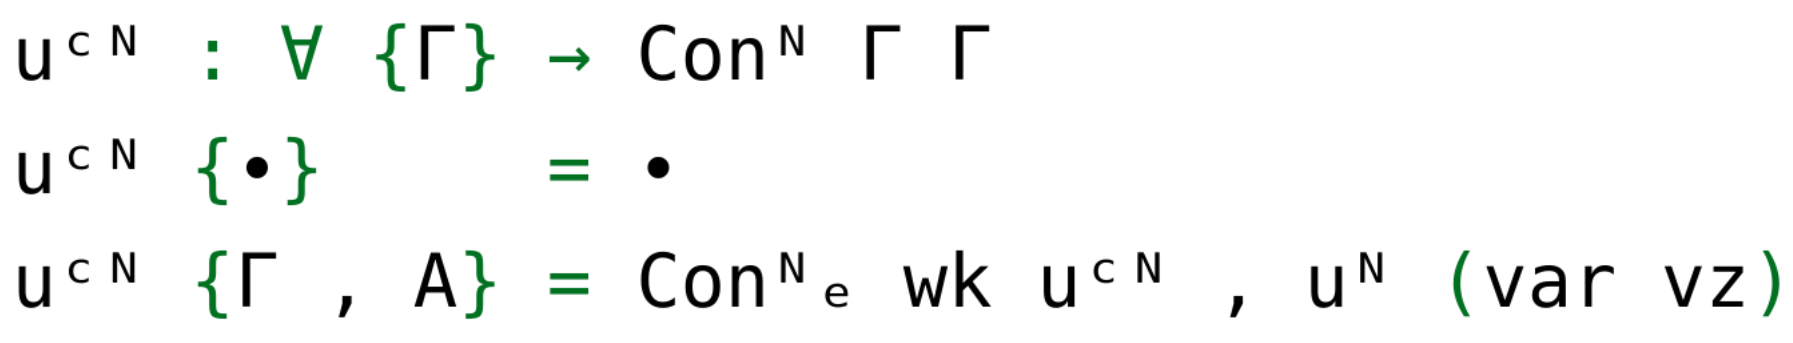
\includegraphics[width=0.6\textwidth]{./images/agda_initial_env.png}
    \caption{Agda implementation of \code{initialEnv} from \cite{AgdaNbe}}
    \label{fig:agdaInitialEnv}
\end{figure}

Before we define \code{normalise}, we need to specify the initial environment to evaluate our expression in. We want \code{normalise} to return a normal form with the same context as the original term. Since \code{eval :: Env ctx ctxV -> Expr ctx ty -> V ctxV ty} and \code{reify :: V ctxV ty -> NormalForm ctxV ty}, we can achieve this by evaluating with an environment of type \code{Env ctx ctx}. The initial environment is a function of the context of the given expression, as seen in Figure \ref{fig:agdaInitialEnv}, where $\text{u}^\text{c N}$ is the Agda function that produces the initial environment.

\begin{lstlisting}
    class SingContext ctx where
        idOpe :: OPE ctx ctx
        bindOpe :: OPE (x:ctx) ctx
        bindOpe = Drop idOpe
        initialEnv :: Env ctx ctx

    instance SingContext '[] where
        idOpe = Empty
        initialEnv = EmptyEnv

    instance (SingContext xs, SingTy x) => SingContext (x:xs) where
        idOpe = Keep idOpe
        initialEnv = ConsEnv (strengthenEnv bindOpe initialEnv) (etaExpand (NeutralVar Head))
\end{lstlisting}

We emulate the type-level pattern match by further extending the \code{SingContext} class with the \code{initialEnv} function. 
For each element in the context, we add a new semantic variable to the environment, strengthening the contexts of all the semantic elements in the environment accordingly using \code{strengthenEnv bindOpe}. This allows us to normalise expressions with free variables where the type of each free variable is given in the context. \code{etaExpand} requires that \code{x} has a \code{SingTy} instance, so we implicitly pass this guarantee by adding a \code{SingTy} constraint to the instance. 

Grouping functions under a single type class like this could be problematic for more complicated applications, as it may lead to an accumulation of class constraints. For example, consider the following \code{hypothetical} function.

\begin{lstlisting}
    hypothetical :: (SingContext ctx) => Expr ctx ty -> OPE (ty:ctx) (ty:ctx)
    hypothetical _ = idOpe
\end{lstlisting}

Even through \code{idOpe} only depends on the length of a context rather than its contents, to use the \code{idOpe} implementation for \code{ty:ctx}, the \code{(:)} instance for \code{SingContext} requires that \code{ty} is a member of \code{SingTy}. Thus, \code{hypothetical} does not type-check and compilation fails. In cases like these it would be necessary to split the type-level pattern-matching functions across distinct classes, to avoid the accumulation of constraints on a single class instance. This could lead to significant amounts of boilerplate in applications using classes for type-level pattern matching more frequently. In our implementation, adding this constraint does not prevent other functions from type-checking. 

\begin{lstlisting}
    normalise :: (SingContext ctx) => Expr ctx ty -> NormalExpr ctx ty
    normalise = reify . eval initialEnv
\end{lstlisting}

The type signature of \code{normalise} is the motivation for all the additional type-level restrictions in this implementation. Given a well-typed expression, \code{normalise} is guaranteed by the type system to return a well-typed normal form with the same context and type as the original expression. The type information in our implementation acts as a proof of this property, which is verified at compile time by the type-checker.

To normalise an expression, the user must specify a concrete context and type for the expression using type annotations. This instantiates type variables which enables polymorphic functions to resolve to specific instances. For example,

\begin{lstlisting}
    normalise (Lam (Var Head) :: Expr '[] (BaseTy :-> BaseTy)) 
        = Lam (Var 0)
\end{lstlisting}

whereas

\begin{lstlisting}
    normalise (Lam (Var Head) :: Expr '[] ((BaseTy :-> BaseTy) :-> BaseTy :-> BaseTy))
        = Lam (Lam (App (Var 1) (Var 0)))
\end{lstlisting}

where the returned terms are expressed in de Bruijn syntax for brevity.

This implementation returns expressions in $\eta$-expaned form as well as $\beta$-normal form, so different type annotations can lead to different terms even if the syntax is the same. 

Below we attempt to normalise a term with a polymorphic type signature.

\begin{lstlisting}
    normalise (Lam (Var Head) :: Expr '[] (a :-> a))
\end{lstlisting}

However, this expression cannot be normalised and GHC produces an error since \code{a} is a type variable. Without a concrete type, GHC is unable to resolve instances of polymorphic functions such as \code{etaExpand} at runtime.

Whilst it is guaranteed that the returned expression of \code{normalise} is normal form, it is not guaranteed that it is the correct normal form for the given expression. Andras Kovacs goes further in his paper and formulates a machine-checked proof of correctness for his implementation of NbE in Agda \cite{AgdaNbe}. It would be interesting to see if this too can be translated into Haskell.

% TODO: Move above to evaluation/conclusion

\section{Notes - IGNORE FOR PROOF READING}

Investigation: Are GADTs in Haskell powerful enough? Types are erased at runtime so true dependent typing not part of Haskell (programs at type level)

Advantage over ADTs: type refinement by constructor

Poissible to erase all type information, NbE on Untyped
Issue: No proof that type preserved 
Solution: Track types as do evaluation - nbe program itself proof that types preserved (subject reduction parallel?)

Started by implementing same as untyped

Main difference in semantics (V := a -> b | Neutral) 
\cite{slides}

problem: Need to strengthen context evaluating body (eval Lam case)
\subsection{Solution: Order Preserving Embeddings (OPEs)}

Following implementation in Agda \cite{AgdaNbe}, agda has full dependent types (type system more powerful) - adapt for haskell, how nicely? 

if a term well typed for one context, also well typed for any longer one

A value of type 'OPE strong weak' can derive weak from strong by dropping elements from context

OPE is a relation on typing contexts

\subsection{Semantic set}

Defintion of V using OPEs - Haskell vs agda

Need to quantify over 'strong' in function - OPE strong weak is guarentee that strong is a stronger context than weak (if quantified at start end up with values where weak stronger than strong) - need rank2 types extension for nested quantification

Helper functions (composition, strengthing relative to OPE) - explain derivations

\subsection{implementing Eval}

Defintion of environment (maps expressions in syntax context ctx to values in semantics with context ctxV)

problem: in app case how to we get identity OPE for semantic context?

But types erased at compile time to make Haskell efficient

How to generate a value at runtime dependent on type erased at compile time

dependent pattern match \cite{SingletonsGuide}

\subsection{Solution: Singleton pattern}

Method of Type to value known as reflection \cite{SingletonsGuide}

Idea: Create value-level tags for types - singleton types correspond type we're interested in, inhabited by only one value for each case

Examples: Reify case analysis, Ty reflection, Context reflection

Explicitly passing as value to pattern match on

Generate implictly using typeclass, use class constraint to imiplictly pass down ability to use contex methods through function calls.
Is it a good idea to have class constraints in the GADTs/Syntax definitions?

Implementation in class vs full reflection - test this for speed?

problem : Inferring Any for ctxV (why?)

solution: scoped type variables - universally quantified variables used in type expressions bind over 'where' clause

(More usefully) can 'unpack' refined GADT types so that can create type definitions using refined types.

Analysis:

Have to specify type when normaling for correct eta-expansion (eta-long form)

Qs:
How does locally nameless work in sematics?
How does ctxV work in Env?
